\begin{document}
The studied strategies were Walk-SAT and GSAT. Even though they were useful for understanding how an incomplete SAT works, our curiosity helps us to find new ones.\\
Our first implementation was the Walk-Sat that we've seen in the class. As it was our first implementation we weren't able to compare it with any other, so we decided to implement gsat in porpouse to see wich one of the two performs better.\\
After this we seen that our implementation of WalkSAT was the way better than the GSAT one.\\
Once we already implemented the two types of SATS that we seen in class, we start searching for a strategy that performs better than this both, and we found one quite interesting.\\
This new one was a combination of the Walksat Random restarts strategy with the functionaity of the GSAT. And that makes a lot of sense for us becouse we thought that GSAT probably was slower due to he stucs a lot more in local minimas than WalkSAT do. This strategy is called Random Walk GSAT.\\
Next in the graphics bellow we will show how the three strategies perform in a set of satisfiable and diferent sized formulas:
\begin{figure}
	\centering
		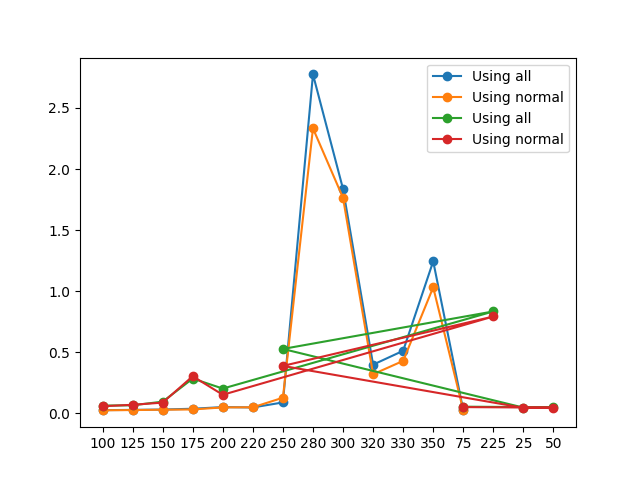
\includegraphics[width=0.7\textwidth]{50-graphic-2.png}
	\caption{Graphic GSAT vs WalkSAT vs Random Walk GSAT }
\end{figure}
\begin{figure}
	\centering
		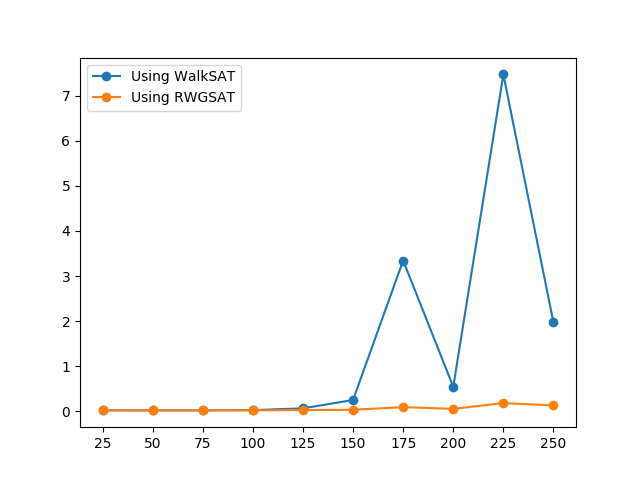
\includegraphics[width=0.7\textwidth]{50-graphic-1.png}
	\caption{Graphic WalkSAT vs Random Walk GSAT }
\end{figure}
\end{document}
